\documentclass{article}
\usepackage{geometry}
\geometry{a4paper, top=3cm, bottom=3cm, left=2cm, right=2cm}
\usepackage[utf8]{inputenc}
\usepackage[english]{babel}
\usepackage{hyperref}
\makeindex

\title{Foundations of Artificial Intelligence\\ Exercises Sheet 8}
\author{Riccardo Salvalaggio}
\date{21th of June, 2021}

\usepackage{amssymb}
\usepackage{amsmath}
\usepackage{txfonts}
\usepackage{mathdots}
\usepackage[classicReIm]{kpfonts}
\usepackage{graphicx}

\begin{document}

\maketitle
\newpage

\textbf{- Exercise 8.1}\\
\begin{itemize}
\item \textbf{(a)}\\\\
Some events were already independent (as said in the last sheet), respectively: E (even) - T (number $\ge 2$) and O (odd) - T are independent. It follows also for the conditionally independence.\\ $P(E \wedge T|U) = P(E|T, U)P(T|U)$\\
Since, E and T are conditionally independent, it follows:\\
$= P(E|U)P(T|U)$, where U (die rolled $\ge$ 2). The same reasoning can be done for O and T.\\
Instead, a case of conditionally dependence (that also follows from the previous sheet) is the following one:\\
$P(E \wedge O|U) =P(E|O, U)P(O|U) = 0\cdot P(o | u) = 0*\frac{2}{5}, $ while, without the conditional event, it would have been: $P(E|U)P(O|U) = \frac{3}{5} \frac{2}{5}$


\item \textbf{(b)}\\\\
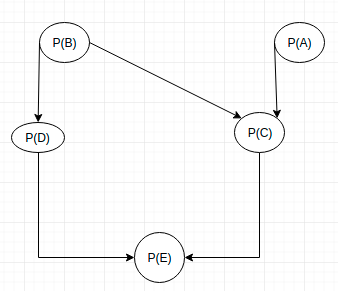
\includegraphics[scale=0.5]{1.png}\\\\
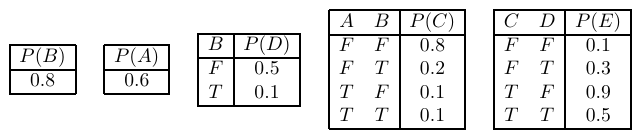
\includegraphics[scale=0.5]{2.png}\\\\
$P(A,\neg B,\neg D, E)$\\
$=P(A|\neg B, \neg D, E)*P(\neg B| \neg D, E)*P(\neg D| E)*P(E)$\\
$=P(A)*P(\neg B)*(\neg D)*P(E)$\\
$=0.6*0.2*0.82*0.266 = 0.026$\\

$P(D) = P(D,B) + P(D,\neg B) = P(D|B)P(B) + P(D|\neg B)P(\neg B)$\\
$= 0.1*0.8 + 0.5*0.2 = 0.18$\\

$P(\neg D) = 1 - P(D) = 0.82$\\

$P(C) = P(C,A,B)+ P(C,\neg A, B) + P(C,A,\neg B)$\\
$P(C) = P(C|A,B)P(A|B)P(B) + P(C|\neg A,B)P(\neg A|B)P(B) + P(C|A,\neg B)P(A|\neg B)P(\neg B) + P(C|\neg A,\neg B)P(\neg A|\neg B)P(\neg B)$\\
$P(C) = 0.1*0.6*0.8 + 0.2*0.4*0.8 + 0.1*0.6*0.2 + 0.8*0.2*0.4 = 0.188$\\

$P(E) = P(E,C,D)+P(E,\neg C,D)+P(E,C,\neg D) =$\\
$= P(E|C,D)P(C|D)P(D) + P(E|\neg C,D)P(\neg C|D)P(D) + P(E|C, \neg D)P(C|\neg D)P(\neg D) + P(E|\neg C, \neg D)P(\neg C|\neg D)P(\neg D)$\\
$P(E) = 0.5*0.188*0.18 + 0.3*0.812+0.18 + 0.9*0.188*0.82 + 0.1*0.812*0.82 = 0.266$

\end{itemize}

\textbf{- Exercise 8.2}\\
\begin{itemize}
\item \textbf{(a)}\\\\
$P(E,E,E,E,N) = P(E|E,E,E,N) \cdot P(E|E,E,N) \cdot P(E|E,N) \cdot P(E|N) \cdot P(N)$\\
Since every event is independent from the previous one:\\
$ = P(E) \cdot P(E) \cdot P(E) \cdot P(E) \cdot P(N)$\\
These are the intended directions (P(intended direction) = 0.8), so:\\
$ = 0.8 \cdot 0.8 \cdot 0.8 \cdot 0.8 \cdot 0.8 = 0.328$.
\item \textbf{(b)}\\\\
With very low probability, every other direction is achievable. The agent will stop if has already done 5 steps, or is in a terminal state.\\\\
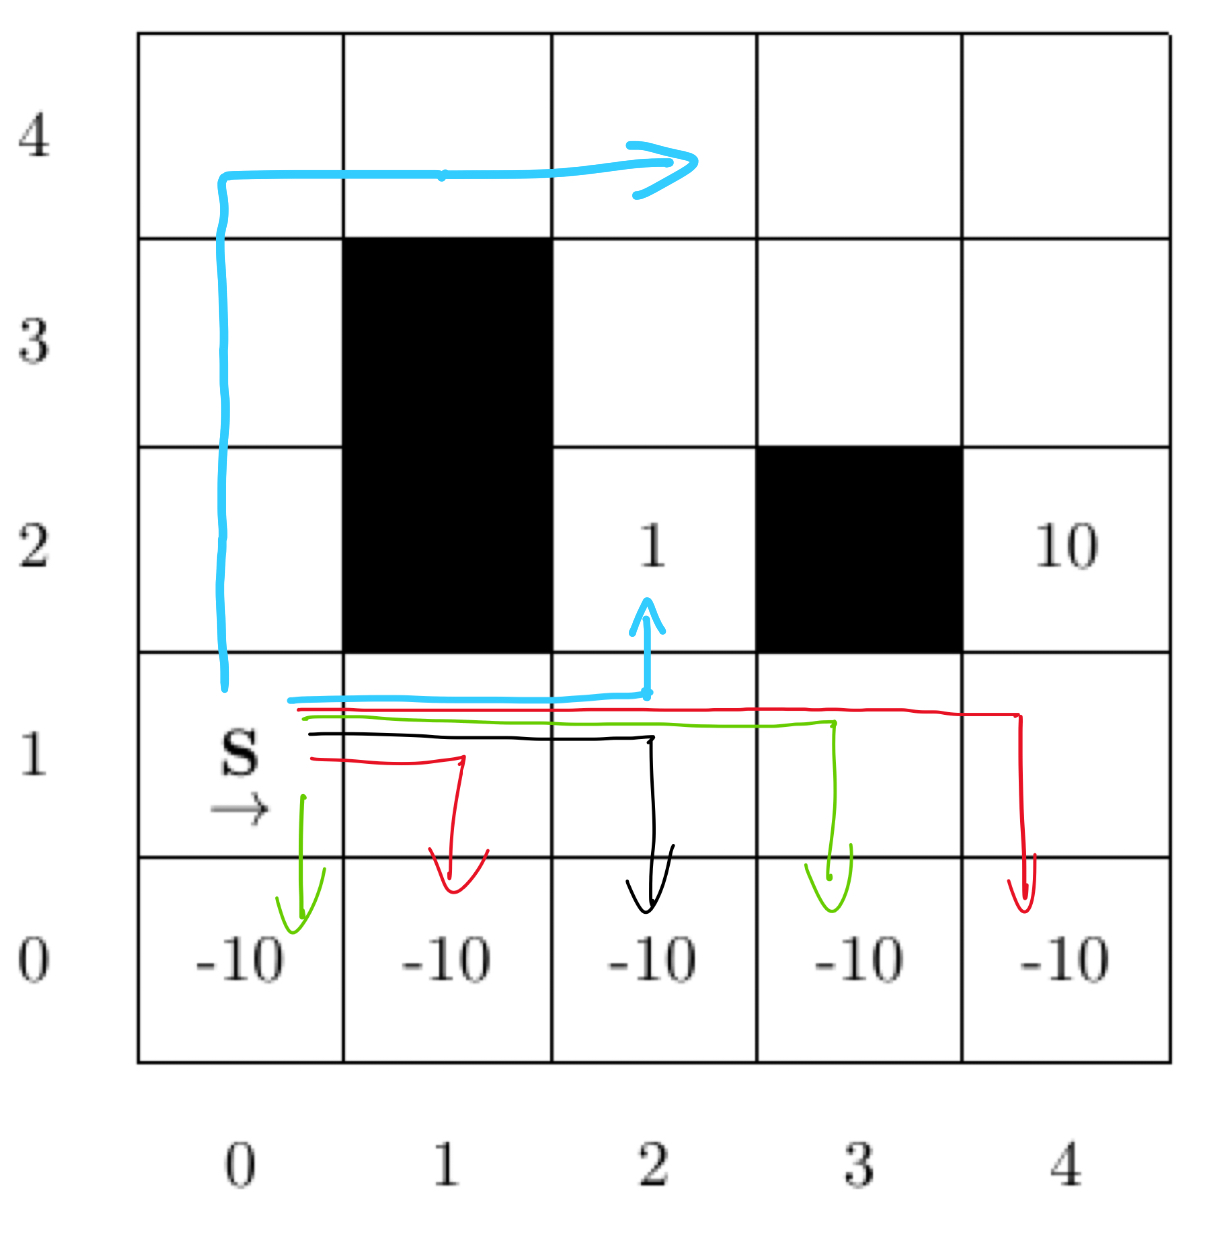
\includegraphics[scale=0.2]{80.JPG}




\end{itemize}

\end{document}
